% !TEX root = article.tex

\section{OSR in LLVM}
\label{se:osr-llvm}

% ====> The following text goes in the artifact
% In this section we discuss our implementation of the approach described in \mysection\ref{se:overview} in \tinyvm, a proof-of-concept virtual machine we developed as a playground to exercise our OSR techniques. TinyVM is based on LLVM's MCJIT compiler and supports interactive invocation of LLVM IR functions either generated at run-time or loaded from disk. The main design goal behind TinyVM is the creation of an interactive environment for IR manipulation and JIT-compilation of functions: for instance, it allows the user to insert OSR points in loaded functions, run optimization passes on them or display their CFGs, repeatedly invoke a function for a specified amount of times and so on. TinyVM supports dynamic library loading and linking, and comes with a helper component for MCJIT that simplifies tasks such as handling multiple IR modules, symbol resolution in presence of multiple versions of a function, and tracking native code and other machine-level generated object such as Stackmaps.

\ifdefined\noauthorea
\begin{figure}[t]
\begin{center}
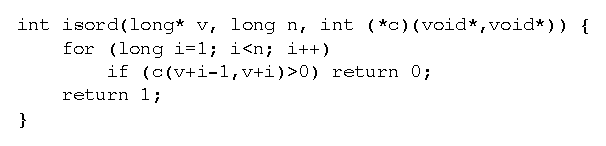
\includegraphics[width=0.9\columnwidth]{figures/isord-example/isord.eps}
\caption{\protect\label{fig:isordfrom} OSR instrumentation of base function in LLVM IR (in grey). The OSR is fired at the beginning of the loop body after 1000 iterations.
}
\end{center}
\end{figure}
\fi

%\subsection{Example}
In this section we discuss one possible embodiment of the OSR approach of \mysection\ref{se:overview} in LLVM. Our discussion is based on a simple running example that illustrates a profile-driven optimization scenario. We start from a simple base function ({\tt isord}) that checks whether an array of numbers is ordered according to some criterion specified by a comparator (see \myfigure\ref{fi:isord-example}). Our goal is to instrument {\tt isord} so that, whenever the number of loop iterations exceeds a certain threshold, control is dynamically diverted to a faster version generated on the fly by inlining the comparator. 

The IR code shown in this section\footnote{Virtual register names and labels in the LLVM-produced IR code shown in this paper have been refactored to make the code more readable.} has been generated with \clang\ and instrumented with \osrkit, a library we prototyped to help VM builders deploy OSR in LLVM. \osrkit\ provides a number of useful abstractions that include open and resolved OSR instrumentation of IR base functions without breaking the SSA (Static Single Assignment) form, liveness analysis, generation of OSR continuation functions, and mapping of LLVM values between different versions of a program along with compensation code generation\footnote{An accompanying artifact will allow the interested reader to get acquainted with \osrkit\ and repeat the sample scenario described in this section.}.

%To explain how the OSR approach of \mysection\ref{se:overview} can be implemented in LLVM, we consider the simple example of \myfigure\ref{fi:isord-example}. Function {\tt isord} checks whether an array of numbers is ordered according to some criterion specified by a comparator.

\ifdefined\noauthorea
\begin{figure}[t]
\begin{center}
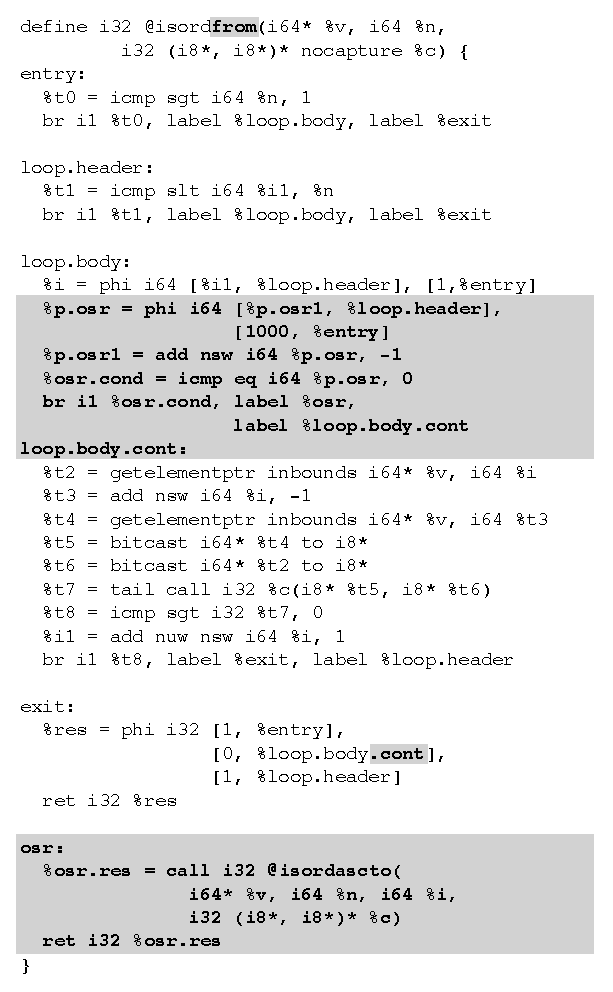
\includegraphics[width=0.9\columnwidth]{figures/isordfrom/isordfrom.eps}
\caption{\protect\label{fig:isordfrom} IR version of base function {\tt isord} (\myfigure\ref{fi:isord-example}) instrumented for resolved OSR. The OSR is fired at the beginning of the loop body after 1000 iterations. Additions resulting from the instrumentation are in grey.
}
\end{center}
\end{figure}
\fi

\ifdefined\noauthorea
\begin{figure}[t]
\begin{center}
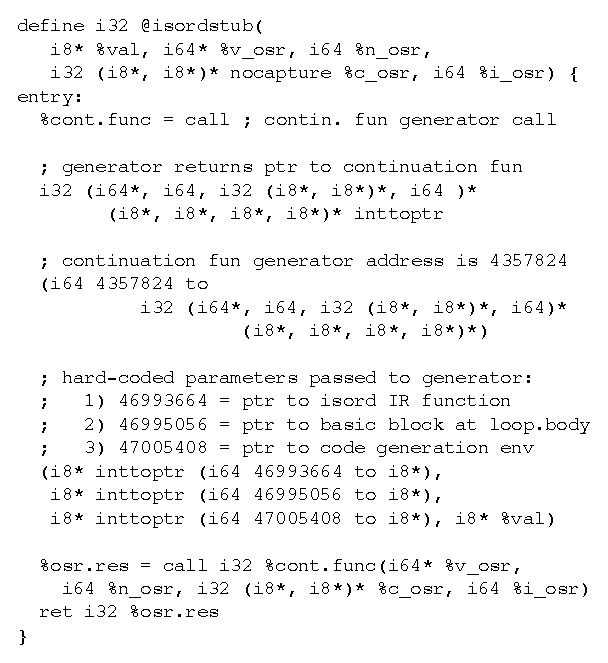
\includegraphics[width=0.9\columnwidth]{figures/isordstub/isordstub.eps}
\caption{\protect\label{fig:isordstub} IR stub that generates the continuation function when an open OSR is fired by {\tt isordfrom} (\myfigure\ref{fig:isordfrom}).
}
\end{center}
\end{figure}
\fi

\ifdefined\noauthorea
\begin{figure}[t]
\begin{center}
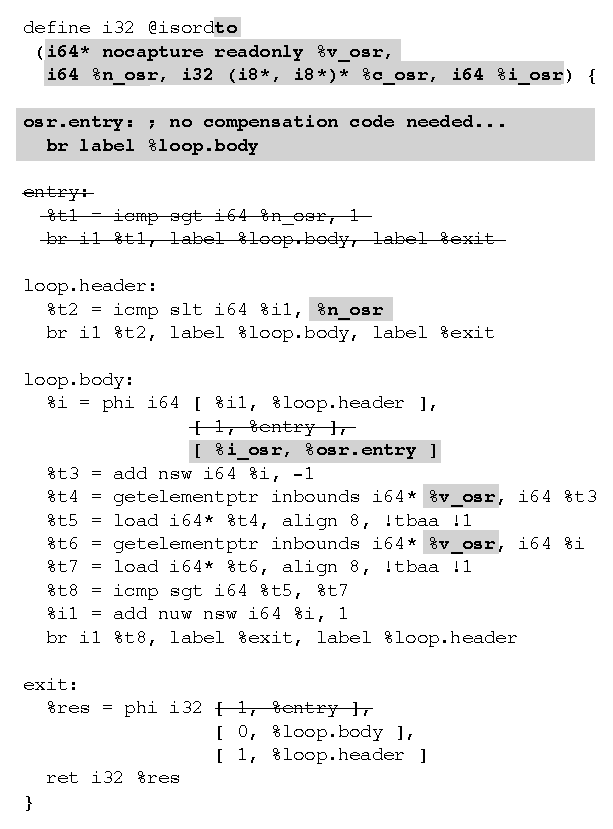
\includegraphics[width=0.9\columnwidth]{figures/isordascto/isordascto.eps}
\caption{\protect\label{fig:isordascto} OSR instrumentation (in grey) of faster variant {\tt isordasc} (\myfigure\ref{fi:osr-dynamics}) in LLVM IR. The original function entry block is unreachable after instrumentation and eliminated (struck-through code fragments).
}
\end{center}
\end{figure}
\fi

\paragraph{OSR Instrumentation in IR.}
To defer the compilation of the continuation function until the comparator is known at run time, we used \osrkit\ to instrument {\tt isord} with an open OSR point at the beginning of the loop body, as shown in \myfigure\ref{fig:isordfrom}. Portions added to the original code by OSR instrumentation are highlighted in grey.
%The figure illustrates how the original {\tt isord} code is instrumented by \tinyvm, highlighting in grey the added portions. 
New instructions are placed at the beginning of the loop body to increment a hotness counter {\tt p.osr} and jump to an OSR-firing block if the counter reaches the threshold (1000 iterations in this example). The OSR block contains a tail call to the target generation stub, which receives as parameters the four live variables at the OSR point ({\tt v}, {\tt n}, {\tt c}, {\tt i}). \osrkit\ allows the stub to receive the run-time value {\tt val} of an IR object that can be used to produce the continuation function -- in our example, the pointer to the comparator function to be inlined. The stub (see \myfigure\ref{fig:isordstub}) calls a code generator that: 1) builds an optimized version of {\tt isord} by inlining the comparator, and 2) uses it to create the continuation function {\tt isordto} shown in \myfigure\ref{fig:isordascto}. The stub passes to the code generator four parameters: 1) a pointer to the {\tt isord} IR code, 2) a pointer to the basic block in {\tt isord} from which the OSR is fired, 3) a user-defined object to support code generation in MCJIT, and 4) the stub's {\tt val} parameter (the first three are hard-wired by \osrkit). The stub terminates with a tail call to {\tt isordto}. To generate the continuation function from the optimized version created by the inliner, \osrkit\ replaces the function entry point, removes dead code, replaces live variables with the function parameters, and fixes $\phi$-nodes accordingly. Additions resulting from the IR instrumentation are in grey, while removals are struck-through.

\ifdefined\noauthorea
\begin{figure}[t]
\begin{center}
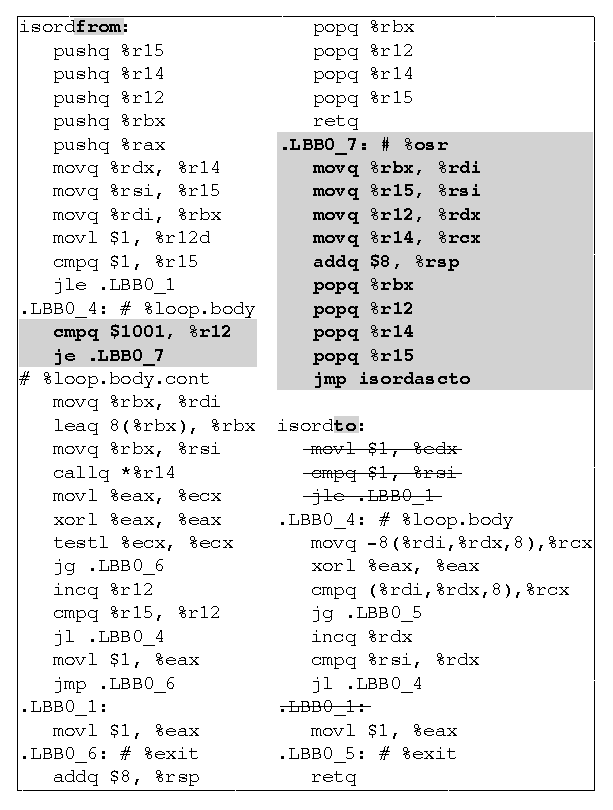
\includegraphics[width=0.9\columnwidth]{figures/isordx86-64/isordx86-64.eps}
\caption{\protect\label{fig:isordx86-64} OSR-instrumented functions {\tt isordfrom} (base) and {\tt isordascto} (faster continuation) after IR to x86-64 lowering in LLVM. For the sake of comparison with the native code that would be generated for the original non-OSR versions, additions resulting from the IR instrumentation are in grey, while removals are struck-through.}
\end{center}
\end{figure}
\fi

\paragraph{x86-64 Lowering.}
\label{se:ir-x86-lowering}

%The final step to be performed before execution is native code generation. 
\myfigure\ref{fig:isordx86-64} shows the x86-64 code generated by the LLVM back-end for {\tt isordfrom} and {\tt isordto}. For the sake of comparison with the native code that would be generated for the original non-OSR versions, additions resulting from the IR instrumentation are in grey, while removals are struck-through. Notice that the OSR intrusiveness in {\tt isordfrom} is minimal, consisting of just two assembly instructions with register and immediate operands. As a result of induction variable canonicalization in the LLVM back-end, loop index {\tt i} and hotness counter {\tt p.osr} are fused in register {\tt\%r12}. We also note that tail call optimization is applied in the OSR-firing block, resulting in no stack growth during an OSR. The continuation function {\tt isordto} is identical to the specialized version of {\tt isord} with inlined comparator, except that the loop index is passed as a parameter in {\tt \%rdx} and no %loop pre-header 
preamble is needed since OSR jumps directly in the loop body.

%\subsection{\osrkit\ Instrumentation API}
%\label{se:instrum-api}
%To support the IR instrumentation tasks of \mysection\ref{se:overview}, \osrkit\ provides a number of abstractions for VM builders. 

%In this section we discuss an LLVM implementation of the approach described in \mysection\ref{se:overview}. Our discussion is based on a set of abstractions to support OSR instrumentation of IR code, which we organized in an LLVM-based library for VM builders called \osrkit. A simplified overview of the main building blocks is:
%\begin{itemize}
%\item {\em StateMapper}: a class that [...]
%\item {\em InsertResolvedOSR(f1, b1, f2, b2, cond, m)}: function that inserts a resolved OSR point in function {\em f1} at basic block {\em b1} to function {\em f2} at basic block {\em b2}, using as OSR condition a sequence of IR instructions {\em cond} and a state mapper {\em m}.
%\item {\em InsertOpenOSR()}: [...]
%\item {\em GenerateOSRContFun(...)}: generates the continuation function [...]
%\end{itemize}

%LLVMContext& Context, OSRLibrary::OpenOSRInfo& info,
%        OSRLibrary::OSRCond& cond, Value* profDataVal, OSRLibrary::DestFunGenerator destFunGenerator,
%        std::vector<Value*> *valuesToTransfer, OSRLibrary::OSRPointConfig &config
%Function* src, BasicBlock* src_bb, std::string* F1NewName, OSRLibrary::OSRCond &cond, int branchTakenProb

%The generated stub calls a function inliner that generates a version of {\tt isord} where the comparator's body, pointed to by live variable {\tt c_osr}, is inlined in the loop body. The optimized version {\tt isordto} is shown in \myfigure\ref{fig:isordascto}.

\paragraph{Comparison with McOSR.}
McOSR~\cite{lameed2013modular} is a library for inserting open OSR points in the legacy LLVM JIT, encoding the OSR machinery entirely in IR as \osrkit\ does. When an OSR is fired, live variables are stored into a pool of globals allocated by the library. McOSR then invokes a user-defined method to transform \fbase\ into \fvariant\ and calls \fbase\ with empty parameters. The new entrypoint of \fbase\ checks a global flag to discriminate if it is being invoked in an OSR transition or as a regular call: in the first case, the state is restored from the pool of global variables before jumping to the OSR landing pad. As the new entrypoint can disrupt LLVM optimizations and lead to poorer performance on subsequent invocations of \fbase, McOSR promptly recompiles \fbase\ after an OSR. However, lessons from the Jikes RVM~\cite{fink2003design} suggest that generating a dedicated function to resume the execution (as  \osrkit\ does with \fosrto) is likely to yield better performance. \osrkit\ improves upon McOSR in a number of aspects, including: 1) support for multiple versions of a function active in memory at the same time; 2) support for resolved OSR and compensation code; 3) insertion of OSR points at arbitrary locations (e.g., at function calls), and not only at loop headers; 4) compatibility with the new MCJIT's design (e.g., a JIT-ted function or module cannot be updated); 5) simpler design that does not require pools of globals to transfer live variables.

%\osrkit\ overcomes a number of limitations of McOSR, including: 1) only one version of a function can be active in memory; 2) there is no provision for resolved OSR points or compensation code; 3) OSR points can be inserted only at loop headers; 4) McOSR relies on features of the legacy JIT (e.g., updating and recompiling a JIT-ted function or module) that are incompatible with MCJIT's design.

